\chapter{Stanovení cíle} \label{goalSettingChapter}

V této kapitole se zamyslíme a stanovíme cíle, o něž tato práce bude usilovat. Následně vybereme nástroje, které nám k dosažení těchto cílů poslouží.  


\section{Jaký chceme výsledek}

\subsection{Zamyšlení}
Čtenář by nyní měl mít za sebou \ref{swordfightingIntroChapter}. kapitolu a měl by tedy mít jisté povědomí, co obnáší boj s chladnou zbraní v reálném světě, a jaké nástrahy nás čekají, kdybychom se ho pokusili zachytit ve videohře. 

V předchozí kapitole jsme si ukázali, že videohry jsou schopny vcelku pěkně zachytit mnoho aspektů, které k boji s chladnou zbraní neodmyslitelně patří - např. důraz na pohyb po bojišti je v akčních videohrách často používaným klišé. Prvkem, který zcela jistě nabízí největší prostor k dalšímu průzkumu, je samotná \textbf{manipulace se zbraní}.

Analyzovali jsme dva zástupce komerčně úspěšných her, které hráči nad zbraní poskytly vcelku značnou kontrolu. Bojové systémy, které obě tyto hry implementovaly, se vyznačovaly tím, že byly výrazně šité na míru zamýšlenému použití - boji proti lidskému protivníkovi. Všechny útoky byly ručně vybrané a animované tak, aby v této situaci fungovaly co nejlépe. Nevýhodou takovéhoto přístupu je velmi nízká flexibilita. Hráči není umožněno meč použít jakýmkoliv jiným způsobem než tím, který tvůrci hry zamýšleli. Rovněž pro tvůrce tento systém činí velmi obtížným přidávání nových, atypických nepřátel. \textbf{Implementace takovéhoto bojového systému se zdá obnášet množství úmorné, programátorsky nezajímavé práce.} Rozhodně zde však najdeme mnoho dílčích prvků, kterými stojí za to se inspirovat.

Protipólem je pak přístup, kdy je umožněn \textbf{plný, ničím neomezený pohyb meče}, dosažený použitím \textbf{realistické fyzikální simulace} namísto ručně vytvářených animací. Příkladem hry, která se o toto pokoušela, bylo \acl{DbtS} (viz \ref{dieByTheSwordDescriptionSubsection}), to je rovněž názorným důkazem, že tato oblast vyžaduje mnoho dalšího výzkumu. V době svého vydání byla hra technologickým zázrakem, v současnosti jsou však její základní stavební kameny (tj. fyzikální simulace a procedurální animace) běžně dostupnými součástmi herních enginů. \textbf{Zkusit naimplementovat něco podobného za použití moderních nástrojů by mohlo být zajímavým úkolem.}

Kamenem úrazu se \acl{DbtS} stalo \textbf{ovládání}, o kvalitě jeho myšlenky nás ale mohou přesvědčit moderní hry s mečem pro VR. V oblasti desktopových her na \acl{DbtS} nikdo nenavázal, protože nebyl vyřešen problém ovládání. Problém ovládání nebyl nikdy vyřešen také proto, že proprietární charakter hry zkrátka neumožnil komunitě živelně experimentovat s odvážnými novými metodami. Nebylo by tedy záslužné, kdyby naše hra \textbf{mohla posloužit jako otevřená platforma, která sofistikované experimenty v této oblasti umožní?} 

\subsection{Rozhodnutí}

Docházíme tedy k závěru, že náš výsledek by měl vnitřně umožnit \textbf{volný pohyb zbraně v prostoru}. Toho dosáhneme využitím nějakého z moderních otevřených systémů pro \textbf{fyzikální simulaci}.

Pro jednoduchost si vybereme jednu konkrétní zbraň, které systém bude ušit na míru. Po krátké úvaze jsme se rozhodli pro \textbf{jedenapůlruční meč}.

Uživateli nabídneme \textbf{ovládání pro myš a klávesnici}. Pokusíme se navrhnout co nejlepší, mělo by být ideálně alespoň na srovnatelné úrovni použitelnosti jako ovládání myší v \acl{DbtS}. Prioritou je však spíše jeho všestrannost a myšlenková uchopitelnost - aby mohlo sloužit jako \textbf{univerzální laťka}, proti které lze dobře srovnávat experimentální alternativy. 

Nejvyšší prioritou je rovněž kvalita a modularita implementačního kódu. Ta musí být na takové úrovni, aby celkově zájemci o interakci s naším systémem nebyli demotivování, rovněž specificky aby bylo umožněno jednoduché přidávání nových experimentálních modulů pro ovládání.

\section{Jaké nástroje použijeme}

Aby mohl být dosažen náš cíl vytvoření otevřené platformy, na které bude docházet k živelnému komunitnímu experimentování, je nutné zařídit pro experimentátory \textbf{co nejnižší vstupní bariéru}. K tomu nám může výrazně napomoci, pokud naše práce bude vycházet ze standardizovaných nástrojů a knihoven, které členové komunity již umí používat.


\bigbreak
Po krátkém zamyšlení jsme se rozhodli k \textbf{vytvoření práce použít herní engine Unity \cite{Unity}.} 
\begin{figure}[h]\centering
    \center
    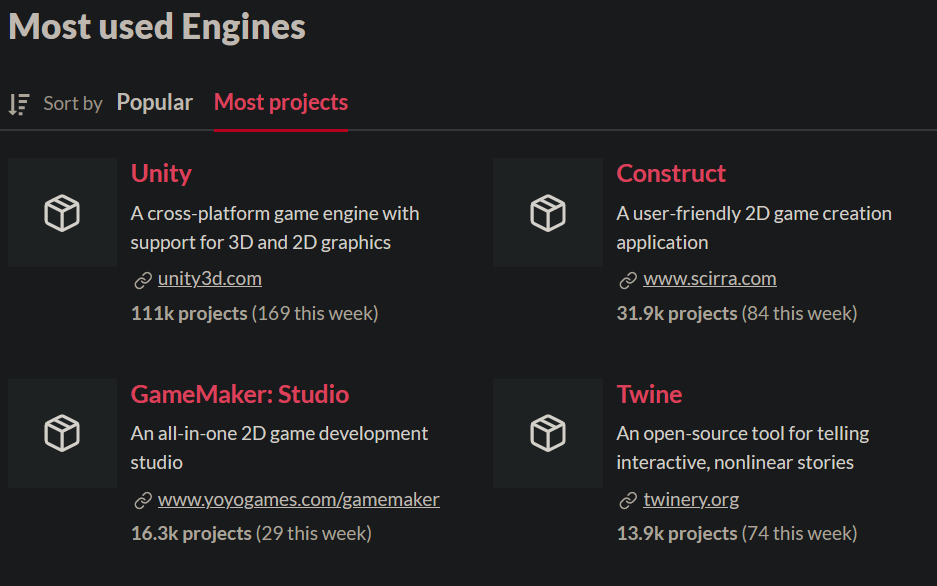
\includegraphics[width=140mm]{../img/Itch-mostUsedEngines.png}
    \caption{itch.io - žebříček používanosti herních enginů - screenshot pořízen 23.4.2023}
    \label{obr02:itchIoEngines}
    
\end{figure}

V době psaní těchto řádek jde dle itch.io \cite{ItchIo} o zdaleka \textbf{nejpoužívanější herní engine}. Tato stránka je oblíbeným místem, kde své hry publikují příležitostní a nezávislí vývojáři - tedy přesně potenciální publikum naší práce. 

Jde o engine, který již za sebou má dlouhé roky nasazení v praxi, během kterých prokázal, že s jeho pomocí lze vytvářet masivní vysokorozpočtové hry i drobné gamejamové\footnote{Pro neznalé: akce, při které se fyzicky či online shromaždí velké množství lidí a po týmech soutěží, kdo během 48 hodin (či podobně drobného časového úseku) vytvoří nejzajímavější hru na vylosované téma.} jednohubky. Rovněž nabízí velmi bohatý \textbf{výběr integrovaných nástrojů} - mimo jiné zde najdeme i pokročilý fyzikální subsystém. Jeho použitím tedy získáme solidní základ, který nám umožní soustředit se na zajímavé aspekty naší práce. Použitím standardních nástrojů jako základů získáme základní míru kompatibility s prací mnoha dalších lidí a maximalizujeme tím množinu těch, kteří by z plodů naší práce mohli těžit.

Jako konkrétní verzi enginu volíme Unity 2022.2. Ač nejde o \acs{LTS} verzi a není tedy zaručena naprostá stabilita, bylo zde přidáno několik velmi drobných rozšíření, která na různých místech usnadní implementaci této práce.  

\section{Shrnutí}
Rozhodli jsme se vytvořit simulátor boje s jedenapůlručním mečem, který vnitřně umožní volný pohyb zbraně v prostoru, uživateli poskytne ovládání pro klávesnici a myš. Jako prostředek k dosažení tohoto cíle použijeme herní engine Unity \cite{Unity} s jeho integrovaným fyzikálním subsystémem. 
